\chapter{解集合プログラミング}\label{chap:asp}


\section{ASP 言語}
解集合プログラミング(ASP; 
\cite{%
  baral03:cambridge,%
  DBLP:conf/iclp/GelfondL88,%
  DBLP:journals/amai/Niemela99})
の言語は, 一般拡張選言プログラムをベースとしている.
本章では, 簡単のため, そのサブクラスである
標準論理プログラムについて説明する. 
以下では, 標準論理プログラムを単に論理プログラムと呼ぶ.
論理プログラムは, 以下の形式のルールの有限集合である.
\begin{displaymath}
  \label{eq:rule}
  a_0\leftarrow a_1,\dots,a_m,\naf{a_{m+1}},\dots,\naf{a_n}
\end{displaymath}
ここで,
$0\leq m\leq n$ であり, 
このルールの直観的な意味は, 
「$a_1,\ldots,a_m$がすべて成り立ち,$a_{m+1},\ldots,a_n$のそれぞれが成
り立たないならば,$a_0$が成り立つ」である.
各$a_i$はアトム, 
$\naf{}$はデフォルトの否定 (述語論理における否定($\neg$)とは意味が異なる), 
``$,$''は連言($\land$)を表す. 
また, $\leftarrow$の左側をヘッド, 右側をボディと呼ぶ. 
ボディが空のルールをファクトと呼び, 
$\leftarrow$を省略して表すことが出来る. 
ヘッドが空のルールを一貫性制約と呼ぶ.

ASP言語には, 組合せ問題を解くために便利な拡張構文が用意されている.
その一例として, 選択子や個数制約がある. 
選択子は\(\{a_1;\dots;a_n\}\)のように表され, アトム集合\(\{a_1,\dots,a_n\}\)の任意の部分集合を表現することが出来る. 
選択子の両端に選択可能な個数の上下限を付けることで, 
任意の部分集合を表していた選択子ではなく, 
アトムの個数が上下限内に収まるような部分集合を表す個数制約となる. 
また, 組合せ最適化問題を解くための最小化関数
(\code{#minimize})や最大化関数(\code{#maximize})も存在する. 
最小化, および最大化したい目的関数は複数記述することが可能であり, 
それぞれに優先度を付けることで優先度の高い目的関数から最適化探索を
行うようにすることも可能である. 
さらに,探索ヒューリスティックスをカスタマイズするための 
\code{#heuristics}文も用意されている.
こちらについては第5章で詳しく説明する.

ASPソルバーは, 与えられた論理プログラムから, 
安定モデル意味論~\cite{DBLP:conf/iclp/GelfondL88}
に基づく解集合を計算するプログラムである. 
近年では, 
{\clingo}~\footnote{\url{https://potassco.org/clingo/}},
{\dlv}~\footnote{\url{http://www.dlvsystem.com/dlv/}},
{\wasp}~\footnote{\url{https://www.mat.unical.it/ricca/wasp/}}
など, SATソルバー技術を応用した高速なASPソルバーが開発されている.
なかでも{\clingo}は, 高性能かつ高機能なASPソルバーとして世界中で広く使
われている. 

% 次に, 解集合の定義について簡単に説明する. 
% 詳細については文献
% \cite{%
%   baral03:cambridge,%
%   DBLP:conf/iclp/GelfondL88,%
%   DBLP:journals/amai/Niemela99}
%  を参考にされたい. 
%  論理プログラム$P$について考える. 
% そして以下に示すような表記を導入する. 
% \begin{itemize}
% \item $\head{r}$ はルール$r$のヘッドを表す
% \item $\pbody{r}$はルール$r$のボディにあるデフォルトの否定が付いていないアト
% ムの集合を表す
% \item $\nbody{r}$はデフォルトの否定が付いているアトムの集合を表す
% \end{itemize}

% 論理プログラム$P$のアトム集合$X$に関するリダクト
% $\reduct{P}{X}$を以下のように定義する. 
% \[\reduct{P}{X}
%   =
%  \{\head{r}\leftarrow\pbody{r} \mid r\in P, \nbody{r}\cap X=\emptyset\}\]
% この時, アトム集合$X$が$\reduct{P}{X}$の最小モデルであるならば, 
% $X$が$P$の解集合となる. 

解集合プログラミングを用いた問題解法のプロセスは, 以下の手順からなる. 
まず最初に, 解きたい問題を論理プログラムとして表現する. 
次に, ASP ソルバーを用いて, 論理プログラムの解集合を計算する. 
最後に, 解集合を解釈して元の問題の解を得る. 


\section{プログラム例}
ここでは, グラフ彩色問題を例として, 解法プロセスの説明を行う. 
ASP ソルバーとしては{\clingo}を用いる. 
以降で示す論理プログラムのソースコードはすべて{\gringo}言語で書かれて
おり, 論理プログラムの説明で用いた記号のソースコード上での
表記法を表~\ref{tbl:map}に示す. 

%%%%%%%%%%%%%%%%%%%%%%%%%%%%%%%%%
\begin{table}[tb]
  \centering
  \begin{tabular}{l|*{4}{p{1cm}}}
    論理プログラム &   $\leftarrow$ & $,$        & $;$        & $\sim$       \\\hline
    ソースコード   &   \texttt{:-}  & \texttt{,} & \texttt{;} & \texttt{not}
  \end{tabular}
  \caption{論理プログラムとソースコードにおける記号の対応}
  \label{tbl:map}
\end{table}

%%%%%%%%%%%%%%%%%%%%%%%%%%%%%%%%%
\begin{figure}[tb]
  \centering
  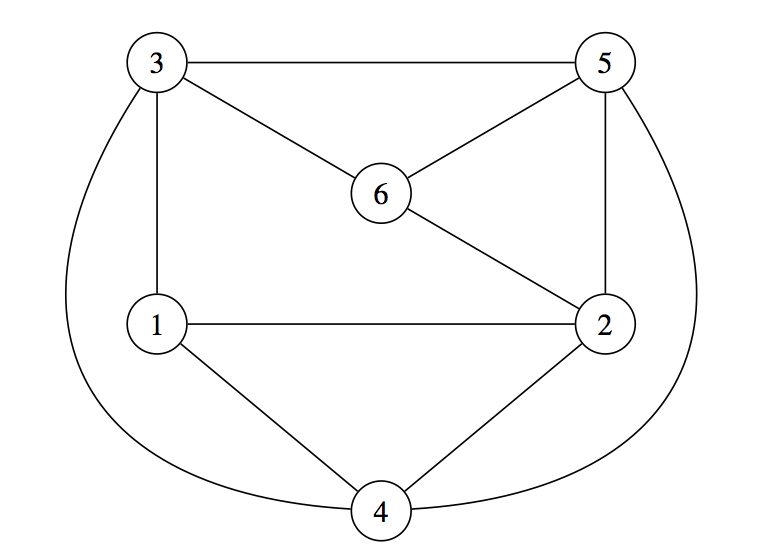
\includegraphics[width=0.6\linewidth]{fig/graph.png}
  \caption{グラフ彩色問題のグラフ}
  \label{fig:graph}
\end{figure}
%%%%%%%%%%%%%%%%%%%%%%%%%%%%%%%%%
\lstinputlisting[float=tb,caption={%
グラフ彩色問題の論理プログラム (\code{color.lp})},%
captionpos=b,frame=single,label=code:color.lp,%
numbers=left,%
breaklines=true,%
columns=fullflexible,keepspaces=true,%
basicstyle=\ttfamily\scriptsize]{code/color.lp}
%%%%%%%%%%%%%%%%%%%%%%%%%%%%%%%%%
\lstinputlisting[float=tb,caption={%
\code{color.lp}に対する{\clingo}の実行例},%
captionpos=b,frame=single,label=code:color.log,%
numbers=left,%
breaklines=true,%
columns=fullflexible,keepspaces=true,%
basicstyle=\ttfamily\scriptsize]{code/color.log}
%%%%%%%%%%%%%%%%%%%%%%%%%%%%%%%%%

グラフ彩色問題とは, 辺で結ばれたノードが同じ色にならないように, 各ノー
ドを塗り分ける問題である. 
図~\ref{fig:graph}のグラフを赤(\code{r}), 青(\code{b}), 緑
(\code{g})の3色で塗り分ける問題を例として用いる. 
この問題を表す論理プログラムをコード~\ref{code:color.lp}に示す. 

1〜3行目は, ノード(\code{node})と辺(\code{edge})をファクトとし
て書くことによって, 図~\ref{fig:graph}のグラフを表している. 
ピリオド(\code{.})はルールの終わりを表す. 
5行目も同様にして, ファクトによって色(\code{col})が表されている. 
%
7行目のルールは, 個数制約を使って, 各ノードが一つの色で塗られるとい
う制約を表している. アトム\code{color(X,C)}は, ノード\code{X}が色
\code{C}で塗られることを意味する. セミコロン(\code{:})は条件付きリテラ
ルと呼ばれる拡張構文で, このルールのヘッドは, 
\code{1 \{ color(X,r);color(X,b);color(X,g) \} 1}のように展開される. 
つまり, ある\code{node(X)}が存在する時, \code{color(X,r),color(X,b),}\\
\code{color(X,g)}
のいずれか一つが真 (いずれか一つの色でXが塗られる) ということになる. 
8行目のルールは, 一貫性制約を使って, 辺で結ばれたノード(\code{X}と
\code{Y})は, 同じ色(\code{C})で塗られないという制約を表している.

ASP ソルバーは解集合を計算して出力する. 
コード~\ref{code:color.log}に{\clingo}の実行例を示す. 
この出力から, ノード1と5は緑, ノード4と6は赤, ノード2と3は青に塗り分け
られることがわかる. 

%\textit{clingo}には, 求解における変数選択ヒューリスティクスの変更を, 
%プログラム上から行うことが出来る機能が存在する. 
%変更には, 論理プログラム上で以下のような表記を用いることで行う. 
%\begin{displaymath}
%\#heuristic \quad A~ : ~Body. ~~~[w,m]
%\end{displaymath}

%これは, \textit{Body}が成り立つ時, アトム $A$ の変数ヒューリスティクスを重み
 %$w$ と指定子 $m$ に従って変更することを表している. 

%変数選択ヒューリスティクスをどのように変更するかは, 指定子によって決定される. 
%本論文では, 指定子として $true$ と $false$ を例にとり説明をする. 
%$true$ はアトムに優先的に真を割り当てるようにする指定子であり, 
%$false$ はアトムに優先的に偽を割り当てるようにする指定子である. 
%例えば, ``\#\textit{heuristic A.} [1,$true$]" は $A$ に優先度レベル1で
%真を優先して割り当てることを表し, 
%``\#\textit{heuristic A : B.} [2,$false$]" は $B$ が真である場合に, 
%$A$ に優先度レベル2で偽を優先して割り当てることを表す. 
%各アトムのデフォルトのレベルは0であり, 
%最もレベルの高いアトムから真もしくは偽が割り当てられる. 

%コード\ref{code:heu.lp}は, \#\textit{heuristic}ルールを用いた
%論理プログラムの例である. 
%1行目には選択子と呼ばれる拡張構文が使用されており, 
%アトム$a$,$b$は真でも偽でも良いということを表している. 
%2行目は一貫性制約を用いて, 
%アトム$a$,$b$が同時に真になってはいけないということを
%表している.  
%3,4行目はそれぞれ$a$,$b$に関する
%\#\textit{heuristic}ルールであり, 
%3行目は, 優先度1で$a$に真を割り当てることを, 
%4行目は, 優先度2で$b$に真を割り当てることを表している. 

%コード\ref{code:heu.log}に\textit{clingo}の実行例を示す. 
%\textit{clingo}では ``--heu=domain" をオプションとして指定することで, 
%\#\textit{heuristic}ルールが有効となる. 
%この実行では, アトム$b$のみが真となった解が出力されている. 
%これは, $a$に関しても真を優先的に割り当てるようなルールが記述されているが, 
%$a$に対するルールが優先度1であるのに対し, $b$に対するルールは優先度2であるので, 
%まず$b$に優先して真が割り当てられる. 
%その後に, 一貫性制約によって$a$,$b$が同時に真になることは禁止されている
%ために$a$に偽が割り当てられ, その結果が出力されている. 
%仮に$a$に関するルールの優先度が3となっていれば, 実行結果は
%$a$のみを含む解が出力される. 
%また, コード\ref{code:heu.lp}で2行目の一貫性制約の記述が無ければ, 
%$a$,$b$どちらの\#\textit{heuristic}ルールも有効となって, 
%実行結果は$a$,$b$の両方を含む解が出力されることになる. 







%%% Local Variables:
%%% mode: japanese-latex
%%% TeX-master: "paper"
%%% End:
